\documentclass[11pt]{amsart}
\usepackage[a4paper,margin=1in]{geometry}
\usepackage{amsmath,amssymb,amsthm}
\usepackage{booktabs}
\usepackage{tikz}
\usetikzlibrary{arrows.meta,positioning}
\usepackage[hidelinks]{hyperref}
\newcommand{\doi}[1]{doi:\href{https://doi.org/#1}{#1}}

\newtheorem{thm}{Theorem}[section]
\newtheorem{lemma}[thm]{Lemma}
\newtheorem{prop}[thm]{Proposition}
\newtheorem{cor}[thm]{Corollary}
\newtheorem{conj}[thm]{Conjecture}
\theoremstyle{definition}
\newtheorem{definition}[thm]{Definition}
\newtheorem{remark}[thm]{Remark}

\newcommand{\Y}{\mathrm{Y}}
\newcommand{\N}{\mathrm{N}}

\title[Even splitting with two and more lies]{Even splitting in the R\'enyi--Ulam game: optimal with two lies,
not with three or more}
\author{Vamshi Jandhyala}
\address{London, United Kingdom}
\date{Preprint, version 2, 24 November 2026 (version 1: 24 November 2026). Not peer reviewed.}
\subjclass[2020]{91A46, 94B60, 68P10, 05A99}
\keywords{R\'enyi--Ulam game, searching with lies, liar game, Berlekamp volume, adaptive search}

\begin{document}

\begin{abstract}
In the R\'enyi--Ulam game one finds an unknown element by yes-or-no questions, and up to $e$ of the answers may be
lies. A position records how many candidates are contradicted by $0,1,\dots,e$ answers. P\'alv\"olgyi conjectured,
while expecting the conjecture to be false, that from a position in which every class has even size it is always
optimal to ask about exactly half of each class. The case $e=1$ is known. We prove the case $e=2$: if the even
position $(2a,2b,2c)$ can be won in $n$ questions, then its halving child $(a,a+b,b+c)$ can be won in $n-1$. The
proof is analytic above depth $15$, where a congruence modulo $\gcd\bigl(n-2,\binom{n-2}2\bigr)$ decides whether the halving
child is winnable and no other first question can avoid that congruence; depths up to $15$ are settled by a finite
certificate checked by two independent programs. For every $e\ge3$ the conjecture is false. For $e=3$, with
$a=(2^{105}-153920)/198592$, the even position $(2a,52,120,0)$ can be won in $106$ questions, but its halving child
$(a,a+26,86,60)$ cannot be won in $105$, although its volume is $2^{105}-28$. The obstruction is a congruence two
questions deep, first modulo $\binom{104}2$ and then modulo $103$; putting $e-3$ empty classes in front gives
a counterexample for every larger $e$. The argument above depth $15$ for $e=2$ and the
obstruction for $e=3$ are formalised in Lean; the winning strategy for $e=3$ is an explicit certificate of $2{,}126$
questions checked by two independent programs.
\end{abstract}

\maketitle

\section{Introduction}

Four people stand in a room and one of them is the culprit. You may ask any yes-or-no question about the culprit,
and the answers may contain up to two lies. How many questions do you need? Each candidate can be ``seen'' along
$1+n+\binom n2$ answer sequences of length $n$ (no lie, one lie in any of $n$ places, two lies in any two places),
and different candidates must be told apart, so $4\bigl(1+n+\binom n2\bigr)\le 2^n$ is necessary. That gives
$n\ge7$. Yet seven questions are not enough; eight are needed. The reason becomes visible after the most natural
first question, ``is the culprit one of these two?'': whatever the answer, two candidates are still allowed two lies
and two have used one, and that position needs seven more questions although its own count promises six.

This is the R\'enyi--Ulam game~\cite{Pelc}. The counting argument is Berlekamp's volume bound~\cite{Berlekamp}, and
the example shows that the bound can fail by one. Halving each class looked like the best opening, and the question
is whether that is always so. P\'alv\"olgyi asked it on MathOverflow in 2014~\cite{MO} and stated it as the first of
three conjectures in a note of the same year~\cite{Palvolgyi}, adding that he expected all three to be false.

To state it, fix the number $e$ of lies. After some questions, a candidate is contradicted by some number $i$ of the
answers; if $i>e$ it is eliminated. A \emph{position} is the vector $(x_0,\dots,x_e)$ of the class sizes, and the
questioner has won when at most one candidate remains. A question is described by how many candidates of each class
it contains, $(q_0,\dots,q_e)$ with $0\le q_i\le x_i$.

\begin{conj}[P\'alv\"olgyi~\cite{MO,Palvolgyi}]\label{conj}
\sloppy If every $x_i$ is even, the even-splitting question $(x_0/2,\dots,x_e/2)$ is optimal: no question leads to a
win in fewer questions in the worst case.
\end{conj}

For $e=0$ this is ordinary binary search. For $e=1$ it follows from the splitting strategy of Ellis, Ponomarenko and
Yan~\cite{EPY}, as P\'alv\"olgyi notes~\cite{MO}. In comments on the question, Zare reported a computer check finding
the conjecture true for at most $52$ candidates and at most three lies. For two lies, Guzicki~\cite{Guzicki}
determined how many questions are needed from every starting position $(N,0,0)$. Along the way he showed that the
pair of opening questions from $(N,0,0)$ that best balances the weights after two answers begins by asking about half
of the candidates \cite[Theorem~4.1]{Guzicki}, and that his typical intermediate positions, under further hypotheses,
are balanced by some question that halves the first class \cite[Theorems~3.3--3.5]{Guzicki}. Those results concern
weight balance and halve only the first class; Conjecture~\ref{conj} asks about winnability from every even position
under the question that halves every class. We settle the case
$e=2$, and show that the conjecture fails for every $e\ge3$.

\begin{thm}\label{thm:main}
Let $e=2$. If the position $(2a,2b,2c)$ can be won in $n\ge1$ questions, then its halving child $(a,a+b,b+c)$ can be
won in $n-1$ questions. In particular, even splitting is optimal at every even position with at least two
candidates.
\end{thm}

\begin{thm}\label{thm:three}
Let $e=3$ and $a=(2^{105}-153920)/198592=204262101229170061472237061$. The even position $(2a,52,120,0)$ can be won in
$106$ questions, and its halving child $(a,a+26,86,60)$ cannot be won in $105$. So the even-splitting question costs
$107$ questions, while the first question $(a,25,112,0)$ wins in $106$.
\end{thm}

\noindent Putting $e-3$ empty classes in front of these positions gives a counterexample for every $e\ge3$
(Corollary~\ref{cor:all}).

The halving child is the position left by either answer to the even-splitting question: a candidate in class $i$
stays in class $i$ if the answer agrees with it and moves to class $i+1$ otherwise, and half of each class goes each
way. The proof of Theorem~\ref{thm:main} is analytic for $n\ge16$ and rests on a finite certificate for $n\le15$
(Section~\ref{sec:base}). Theorem~\ref{thm:three} is proved in Section~\ref{sec:three}.

\subsection*{The idea}
Any question splits the position $x$ into a yes-child $\Y$ and a no-child $\N$, and coordinate by coordinate
$\Y+\N=2h$, where $h$ is the halving child (Figure~\ref{fig:mid}). So the halving child is the midpoint of every pair
of children, and Theorem~\ref{thm:main} says that when both ends of such a pair are winnable, so is the midpoint.
Volume is linear, and the midpoint always satisfies the volume bound when the ends do. What can go wrong is finer: we
show that for the positions that matter the obstruction to winning is a single congruence, and that moving from the
midpoint to an end of the pair cannot repair it, because the shift in volume and the shift in the last class agree
modulo $g=\gcd\bigl(n-2,\binom{n-2}2\bigr)$, for a parent at depth $n$, and are too small to differ by a multiple of $g$.

With three lies the same kind of congruence still blocks the halving child, but it can sit one question deeper,
where the volume test alone does not see it. A first question that keeps the two children's volumes equal yet moves
candidates of the last class from one child to the other changes what the children face at that deeper question,
and in the example of Theorem~\ref{thm:three} this is enough to escape.

\begin{figure}[t]
\centering
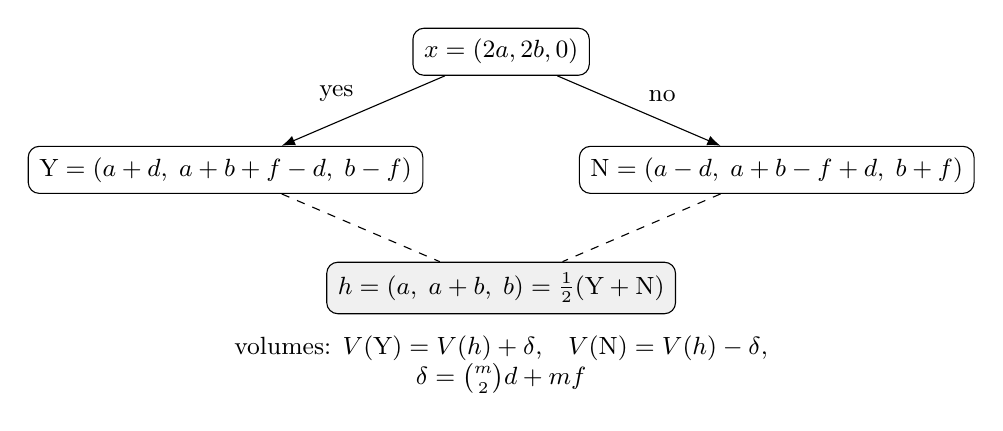
\begin{tikzpicture}[node distance=1.1cm and 2.2cm, every node/.style={font=\small},
  st/.style={draw,rounded corners,inner sep=4pt}]
\node[st] (x) {$x=(2a,2b,0)$};
\node[st] (Y) at (-3.5,-1.5) {$\Y=(a+d,\;a+b+f-d,\;b-f)$};
\node[st] (N) at (3.5,-1.5) {$\N=(a-d,\;a+b-f+d,\;b+f)$};
\node[st,fill=black!6] (h) at (0,-3) {$h=(a,\;a+b,\;b)=\tfrac12(\Y+\N)$};
\draw[-{Latex}] (x) -- node[above left]{yes} (Y);
\draw[-{Latex}] (x) -- node[above right]{no} (N);
\draw[dashed] (Y) -- (h); \draw[dashed] (N) -- (h);
\node[below=0.15cm of h, align=center] {volumes: $V(\Y)=V(h)+\delta$,\quad $V(\N)=V(h)-\delta$,\\
$\delta=\binom m2 d+mf$};
\end{tikzpicture}
\caption{A first question $(a+d,b+f,0)$ from an even position, and the halving child as the midpoint of its two
children. The proof shows that if $h$ is not winnable then $\delta\equiv f\pmod g$ with $|\delta-f|<g$, so
$\delta=f$, and a winning strategy for $\Y$ or $\N$ would hand $h$ exactly what it lacks.}\label{fig:mid}
\end{figure}

\section{Positions, questions and volume}\label{sec:setup}

From now on $e=2$, and a position is a triple $(a,b,c)$: $a$ candidates contradicted by no answer, $b$ by one and $c$
by two. A question $(u,v,w)$ with $u\le a$, $v\le b$, $w\le c$ has children
\[
\Y=\bigl(u,\;v+(a-u),\;w+(b-v)\bigr),\qquad \N=\bigl(a-u,\;(b-v)+u,\;(c-w)+v\bigr).
\]
We call a position \emph{$n$-winnable} if the questioner can win from it within $n$ questions. Put
\[
W_n=1+n+\binom n2,\qquad V_n(a,b,c)=W_na+(n+1)b+c .
\]
Read in words, $V_n$ counts the answer sequences of length $n$ along which some candidate remains possible: $W_n$ for
a candidate that may still be lied about twice, $n+1$ for one that may be lied about once, $1$ for one that may not.
Pascal's rule gives $V_{n+1}(x)=V_n(\Y)+V_n(\N)$ for every question, and induction gives Berlekamp's bound: an
$n$-winnable position has $V_n\le2^n$.

\begin{lemma}[Padding]\label{lem:pad}
If $(a,b,0)$ is $n$-winnable and $V_n(a,b,c)\le2^n$, then $(a,b,c)$ is $n$-winnable.
\end{lemma}

\begin{proof}
Extend a winning strategy for $(a,b,0)$ to depth exactly $n$. A candidate that can still be lied about $r$ times is
consistent with exactly $\sum_{j\le r}\binom nj$ leaves, one for each set of at most $r$ lie positions, and distinct
candidates use disjoint leaves because the strategy wins. So $2^n-V_n(a,b,0)\ge c$ leaves are unused. Send each of
the $c$ added candidates, which can no longer be lied about, down its own unused leaf by putting it in each question
exactly when its leaf's next answer is yes. The original candidates' paths do not change.
\end{proof}

\noindent Lemma~\ref{lem:pad} is Guzicki's Lemma~3.11~\cite{Guzicki}, which adds one candidate to the last class,
applied $c$ times; the leaf-counting proof above is included to keep the note self-contained.

Deleting candidates never hurts, so for each $a$ the $b$ with $(a,b,0)$ $n$-winnable form an initial segment. Write
$B_n(a)$ for its largest element ($-1$ if there is none). By Lemma~\ref{lem:pad},
\begin{equation}\label{eq:frontier}
(a,b,c)\ \text{is $n$-winnable}\iff b\le B_n(a)\ \text{and}\ V_n(a,b,c)\le2^n .
\end{equation}
It is therefore enough to prove Theorem~\ref{thm:main} for $c=0$: if $(2a,2b,2c)$ is $n$-winnable, so is $(2a,2b,0)$;
once $(a,a+b,b)$ is $(n-1)$-winnable, conservation of volume gives $V_{n-1}(a,a+b,b+c)=\tfrac12V_n(2a,2b,2c)\le2^{n-1}$,
and Lemma~\ref{lem:pad} adds the $c$.

\section{Many candidates that can no longer be lied about}\label{sec:lem2}

\begin{lemma}\label{lem:many}
Let $n\ge12$. If $b\ge a$, $c\ge\binom n2$ and $V_n(a,b,c)\le2^n$, then $(a,b,c)$ is $n$-winnable.
\end{lemma}

\noindent This also follows from Guzicki's Theorem~3.9~\cite{Guzicki}: after padding to volume $2^n$, the position
has character exactly $n$ in his sense, since $W_na+(n+1)b<2^n$ forces $na+b<2^{n-1}$, and it is typical
($b\ge a-1$, $c\ge n$), so it is won in $n$ questions. The direct proof below, which reduces to depth $12$, is the
one formalised in Lean.

\begin{proof}
For $n=12$ this is a finite statement, checked in Section~\ref{sec:base}. Let $n\ge13$ and assume the lemma at depth
$n-1$. Adding candidates to the last class, we may assume $V_n(a,b,c)=2^n$; deleting them again at the end is
harmless. Write $D=\binom{n-1}2$, $C=\binom n2$, $H=2^{n-1}$, and note $W_n-D=2n$. For a question $(u,v,w)$ the
yes-child has volume
\begin{equation}\label{eq:yesvol}
V_{n-1}(\Y)=na+b+Du+(n-1)v+w .
\end{equation}
We choose a question with both children of volume exactly $H$, each with middle coordinate at least its first and last
coordinate at least $D$; induction then wins both. Put $u=\lfloor a/2\rfloor$ and $\epsilon=a-2u$.

If $b\ge n$, let $v$ be a nearest integer to $v_*=b/2+\epsilon D/(2n)$ and define $w$ by $V_{n-1}(\Y)=H$ in
\eqref{eq:yesvol}. With $r=v-v_*$, the full-volume equation shows that the two last coordinates are
$\tfrac{b+c}2\mp nr$ and that $w=\tfrac c2+\tfrac{\epsilon D}{2n}-(n-1)r$, so $0\le w\le c$ and $0\le v\le b-1$. The
middle-minus-first differences of the children are $\epsilon+v$ and $b-v-\epsilon$, both nonnegative. Finally
$b+c\ge C+(2^n-C)/(W_n+n+1)\ge2D+n$, the last step being $2^n\ge(W_n+n+1)(D+1)+C$, which holds at $n=13$
($8192\ge7180$) and doubles faster than its right-hand side afterwards. So both last coordinates are at least $D$.

If $b<n$, take $v=\lfloor b/2\rfloor$, $\eta=b-2v$, and $w=\tfrac12(c+\epsilon D+\eta(n-1))$, an integer because the
total volume is even. Both child volumes equal $H$, the children's last coordinates are
$\tfrac12(b+c\pm(\epsilon D+\eta n))$, and $c\ge2^n-(W_n+n+1)(n-1)\ge n^3$ makes both at least $D$. The middle
coordinates dominate the first as before.
\end{proof}

\section{When is the halving child winnable?}\label{sec:crit}

Fix $m\ge15$ and consider $z=(a,a+b,b)$, the halving child of $(2a,2b,0)$, with $s=2^m-V_m(z)\ge0$. Put
\[
D=\binom{m-1}2,\qquad g=\gcd(m-1,D),\qquad K=(m+1)a+b,\qquad H=2^{m-1}.
\]
Explicitly $g=m-1$ for even $m$ and $g=(m-1)/2$ for odd $m$.

\begin{lemma}\label{lem:crit}
$z$ is $m$-winnable if and only if there are integers $t\in[H-s,H]$ and $w\in[0,b]$ with $t\equiv K+w\pmod g$;
equivalently, $(H-K)\bmod g\le s+b$.
\end{lemma}

The integer $t$ is the volume of the yes-child of the first question and $w$ is how many candidates of the last class
that question contains. Both children must have volume at most $H$, which places $t$ in $[H-s,H]$.

\begin{proof}
\emph{Necessity.} By \eqref{eq:yesvol} at depth $m$, a first question $(u,v,w)$ from $z$ has yes-volume
$t=K+Du+(m-1)v+w\equiv K+w\pmod g$, with $0\le w\le b$, and $t\in[H-s,H]$ if both children satisfy the volume bound.
As $w$ ranges over $[0,b]$ and $t$ over $[H-s,H]$, the differences $t-w$ fill $[H-s-b,H]$, which contains a number
congruent to $K$ exactly when $(H-K)\bmod g\le s+b$.

\emph{Sufficiency.} If $b+s\ge\binom m2$, raise the last coordinate of $z$ to $\binom m2$ and apply
Lemma~\ref{lem:many}. Otherwise $V_m(z)=(W_m+m+1)a+(m+2)b$ and $2^m\ge(W_m+m+1)m^2+(m+2)\binom m2$ for $m\ge15$ force
$a\ge m^2$. Take $u$ within $1$ of $a/2$ with the parity (needed only for odd $m$) that makes $t-K-Du-w$ divisible by
$m-1$, and set $v=(t-K-Du-w)/(m-1)$. A short estimate gives $|v-(a+b)/2|<3m/4$, so the question is legal and both
children have middle coordinate at least their first and last coordinate at least $\tfrac{m^2}2-\tfrac{3m}4\ge D$.
Their volumes are $t$ and $V_m(z)-t$, both at most $H$. Lemma~\ref{lem:many} at depth $m-1$ wins both.
\end{proof}

\section{No first question avoids the congruence}\label{sec:key}

\begin{proof}[Proof of Theorem~\ref{thm:main} for $n\ge16$]
By Section~\ref{sec:setup} we may take the parent to be $x=(2a,2b,0)$, $n$-winnable with $n=m+1\ge16$. Suppose its
halving child $z=(a,a+b,b)$ were not $m$-winnable. Then the criterion of Lemma~\ref{lem:crit} fails, and since a
residue is at most $g-1$,
\begin{equation}\label{eq:small}
s+b<g .
\end{equation}
Take the first question of a winning strategy for $x$ and write it as $(a+d,b+f,0)$ with $|f|\le b$. Its children
$\Y$ and $\N$ are shown in Figure~\ref{fig:mid}, and a direct calculation gives
\[
V_m(\Y)=2^m-s+\delta,\qquad V_m(\N)=2^m-s-\delta,\qquad \delta=\tbinom m2d+mf .
\]
Both children are $m$-winnable, so $|\delta|\le s$. Since $g$ divides $\binom m2$ and $m\equiv1\pmod g$, we have
$\delta\equiv f\pmod g$, and by \eqref{eq:small} $|\delta-f|\le s+b<g$. Hence $\delta=f$.

Suppose $f\ge0$ and look at the first question of a winning strategy for $\Y$. By \eqref{eq:yesvol} its yes-volume
$t_\Y$ lies in $[H-s+f,H]$, is congruent to $K+f+w_\Y$ modulo $g$, and $0\le w_\Y\le b-f$. Then $t=t_\Y-f$ and
$w=w_\Y$ satisfy the criterion of Lemma~\ref{lem:crit} for $z$, a contradiction. If $f<0$, the same argument with
$\N$ and $t=t_\N+f$ applies.
\end{proof}

The example from the introduction shows the mechanism at small depth: for four candidates the halving child
$(2,2,0)$ has volume $58\le2^6$ at depth $6$ but needs seven questions, and every other first question from $(4,0,0)$ leaves
a child that is at least as hard.

\section{Small depths}\label{sec:base}

For $n\le15$ we use the frontiers $B_n$ of \eqref{eq:frontier}. With $p=W_{n-1}$ and $H=2^{n-1}$, a question $(u,v,0)$
from $(a,b,0)$ leaves two winnable children exactly when $u$ and $a-u$ are feasible and some integer $v$ satisfies
\begin{multline*}
\max\Bigl(0,\,u+b-B_{n-1}(a-u),\,\Bigl\lceil\tfrac{pa+(n-p)u+nb-H}{n-1}\Bigr\rceil\Bigr)\\
\le v\le\min\Bigl(b,\,B_{n-1}(u)-a+u,\,\Bigl\lfloor\tfrac{H-(p-n)u-na-b}{n-1}\Bigr\rfloor\Bigr),
\end{multline*}
by \eqref{eq:frontier} applied to both children. Starting from $B_0=B_1=(1,0)$ this determines $B_2,\dots,B_{15}$.
The certificate lists these $645$ integers. For each recorded pair it checks winnability at $b=B_n(a)$, failure at
$b=B_n(a)+1$, and failure for the first omitted $a$, so an over- or underestimate cannot pass. It then checks
\[
\bigl\lfloor B_n(2a)/2\bigr\rfloor\le B_{n-1}(a)-a\qquad(1\le n\le15),
\]
which is Theorem~\ref{thm:main} at these depths by \eqref{eq:frontier}, and the $44$ boundary cases of
Lemma~\ref{lem:many} at $n=12$. Table~\ref{tab:frontier} shows the shape of the frontiers.

The certificate was produced and checked with one program and recomputed with a second, written separately, that
searches the game tree directly from the definition of a position and a question, without using the recurrence above.
The two agree on all $645$ values.

\begin{table}[h]
\centering\small
\begin{tabular}{@{}l*{8}{c}@{}}
\toprule
$n$ & 8 & 9 & 10 & 11 & 12 & 13 & 14 & 15\\
\midrule
largest $a$ with $B_n(a)\ge0$ & 4 & 8 & 16 & 28 & 50 & 88 & 154 & 270\\
$B_n(0)$ & 28 & 50 & 92 & 170 & 314 & 584 & 1092 & 2048\\
\bottomrule
\end{tabular}
\caption{Frontiers of the two-lie game. $B_n(0)$ is the largest number of once-contradicted candidates, with no
uncontradicted ones, that can be resolved in $n$ questions.}\label{tab:frontier}
\end{table}

\section{Three lies: a counterexample}\label{sec:three}

From now on $e=3$. A position is $x=(x_0,x_1,x_2,x_3)$, a question $(q_0,\dots,q_3)$ with $0\le q_i\le x_i$, and a
candidate moves up one class when the answer disagrees with it, so the yes-child is
$\Y_i=q_i+(x_{i-1}-q_{i-1})$ (with $x_{-1}=q_{-1}=0$) and the no-child is the same with $x-q$ in place of $q$. Put
\[
W_i(n)=\sum_{j\le3-i}\binom nj,\qquad V_n(x)=\sum_{i=0}^3x_iW_i(n).
\]
Pascal's rule gives $V_{n+1}(x)=V_n(\Y)+V_n(\N)$, hence Berlekamp's bound $V_n\le2^n$ for an $n$-winnable
position, and the proof of Lemma~\ref{lem:pad} applies word for word: if $(x_0,x_1,x_2,0)$ is $n$-winnable and
$V_n(x)\le2^n$, then $x$ is $n$-winnable. Since $W_i(n-1)-W_{i+1}(n-1)=\binom{n-1}{3-i}$, the yes-child of a question
$q$ from $x$ at depth $n$ has volume
\begin{equation}\label{eq:yes3}
V_{n-1}(\Y)=K+\tbinom{n-1}3q_0+\tbinom{n-1}2q_1+(n-1)q_2+q_3,\qquad K=\sum_{i=0}^2x_iW_{i+1}(n-1).
\end{equation}

\begin{lemma}\label{lem:next}
Let $z$ be $m$-winnable with at least two candidates, let $\sigma=2^m-V_m(z)$, and let $g$ divide $\binom{m-1}3$,
$\binom{m-1}2$ and $m-1$. Then, with $K$ as in \eqref{eq:yes3} for $z$ at depth $m$,
\[
\bigl(2^{m-1}-K\bigr)\bmod g\ \le\ \sigma+z_3 .
\]
\end{lemma}

\begin{proof}
Take the first question of a winning strategy. Both children satisfy the volume bound at depth $m-1$ and their
volumes add up to $2^m-\sigma$, so the yes-volume is $2^{m-1}-\ell$ with $0\le\ell\le\sigma$. By \eqref{eq:yes3} it
is congruent to $K+q_3$ modulo $g$. So $2^{m-1}-K\equiv\ell+q_3$, and $0\le\ell+q_3\le\sigma+z_3$.
\end{proof}

\begin{proof}[Proof that the halving child loses]
Let $h=(a,a+26,86,60)$. Since $198592a=2^{105}-153920$,
\[
V_{105}(h)=198592a+153892=2^{105}-28 ,
\]
so the volume bound leaves a slack of $28$. Suppose a question $(u,v,w,t)$ begins a winning $105$-question
strategy, with $w\le86$ and $t\le60$. At depth $104$ the increments in \eqref{eq:yes3} are
$\binom{104}3=182104=34\cdot5356$, $\binom{104}2=5356$, $104$ and $1$, and $K=5566a+2816$. The yes-volume is
$2^{104}-\lambda$ with $0\le\lambda\le28$, and $(2^{104}-K)\bmod5356=1838$, so
\[
104w+(t+\lambda)\equiv1838\pmod{5356},\qquad 0\le104w+t+\lambda\le104\cdot86+88=9032 .
\]
The left side is therefore $1838$ or $7194$, and as $0\le t+\lambda\le88$ the only possibilities are
\begin{equation}\label{eq:twocases}
(w,\,t+\lambda)=(17,70)\quad\text{or}\quad(69,18).
\end{equation}
The children are
\[
\Y=(u,\;a-u+v,\;a+26-v+w,\;86-w+t),\qquad\N=(a-u,\;a+26-v+u,\;86-w+v,\;60-t+w).
\]
Both are $104$-winnable, and their slacks at depth $104$ are $\lambda$ and $28-\lambda$. Apply Lemma~\ref{lem:next} to each with $m=104$ and $g=103$,
which is prime and so divides $\binom{103}3$, $\binom{103}2$ and $103$. Modulo $103$ the constants are
$K_\Y\equiv2a+26+w$ and $K_\N\equiv2a+9-w$, independent of $u$ and $v$, and $2^{103}-2a-26\equiv35$,
$2^{103}-2a-9\equiv52$. The lemma requires
\[
(35-w)\bmod103\le\lambda+86-w+t,\qquad(52+w)\bmod103\le(28-\lambda)+60-t+w .
\]
In the first case of \eqref{eq:twocases} the no-child needs $69\le35$; in the second the yes-child needs $69\le35$.
Both are impossible, so $h$ is not $105$-winnable.
\end{proof}

\begin{figure}[t]
\centering
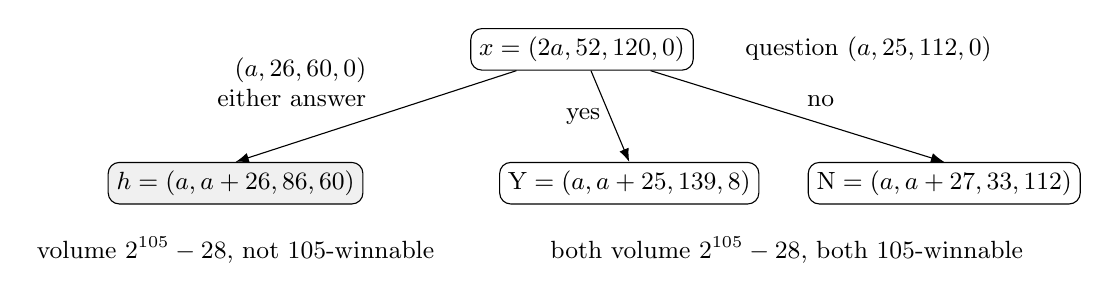
\begin{tikzpicture}[every node/.style={font=\small}, st/.style={draw,rounded corners,inner sep=3pt}]
\node[st] (x) at (0,0) {$x=(2a,52,120,0)$};
\node[st,fill=black!6] (h) at (-4.4,-1.7) {$h=(a,a+26,86,60)$};
\node[st] (Y) at (0.6,-1.7) {$\Y=(a,a+25,139,8)$};
\node[st] (N) at (4.6,-1.7) {$\N=(a,a+27,33,112)$};
\draw[-{Latex}] (x) -- node[above left,align=right]{$(a,26,60,0)$\\ either answer} (h.north);
\draw[-{Latex}] (x) -- node[left]{yes} (Y.north);
\draw[-{Latex}] (x) -- node[above right]{no} (N.north);
\node[anchor=west] at (1.95,0) {question $(a,25,112,0)$};
\node[align=center] at (-4.4,-2.55) {volume $2^{105}-28$, not $105$-winnable};
\node[align=center] at (2.6,-2.55) {both volume $2^{105}-28$, both $105$-winnable};
\end{tikzpicture}
\caption{The counterexample of Theorem~\ref{thm:three}. The even split sends both answers to $h$. The question
$(a,25,112,0)$ shifts volume by $-\binom{105}2+105\cdot52=0$, so its children have the same volume as $h$, but it
moves $52$ candidates of the last class from one side to the other, and both children can be won.}\label{fig:three}
\end{figure}

\subsection*{The winning side} Theorem~\ref{thm:three} also needs $x=(2a,52,120,0)$ to be $106$-winnable. This is
certified by a list of $2{,}126$ rows $(n,y,q)$, each naming a position $y$ at depth $n$ and a question $q$, including
the row $(106,x,(a,25,112,0))$; its children are shown in Figure~\ref{fig:three}. A checker verifies, row by row
in increasing depth, that $q$ is legal, that $V_n(y)\le2^n$, and that each child satisfies the volume bound at depth
$n-1$ and either has at most one candidate in its first three classes or has those three classes equal to a row
already certified at depth $n-1$. By the padding lemma above, every row's position is then winnable. The $631$ rows at
depth at most $18$ come from an exact search. Of the rows at larger depths, all but six halve each of the first three
classes, rounding down, and choose the last-class count to make the two volumes equal; the six exceptions are the
root, the two children $\Y$ and $\N$ at depth $105$ and three positions at depth $104$, whose questions were found by
a search near the root. The checker verifies every row as it stands and assumes no rule. Two checkers, written separately and sharing no code, accept the list, and each rejects it
when the root question is changed or a row is deleted. As $V_{105}(x)>2^{105}$, the parent needs exactly $106$
questions. The list also certifies $h$ at depth $106$, so $h$ needs exactly $106$.

\begin{cor}\label{cor:all}
Conjecture~\ref{conj} is false for every $e\ge3$.
\end{cor}

\begin{proof}
For $e\ge3$, put $e-3$ zeros in front of the positions of Theorem~\ref{thm:three}, so that their candidates are the
last four classes, with $3,2,1,0$ lies left as before. A question cannot contain candidates of an empty class, and no
candidate can enter class $i\le e-3$, since that would need one from class $i-1$, so the leading classes stay empty
in every position reached. The game from these positions is therefore the three-lie game, move for move, and the
even position $(0,\dots,0,2a,52,120,0)$ can be won in $106$ questions while its halving child needs $106$.
\end{proof}

\subsection*{Why the two-lie argument does not carry over} Section~\ref{sec:key} used that a non-halving first
question shifts the children's volumes by $\delta\equiv f$ modulo $g$, and that the halving child's failure forces
$s+b<g$, so that $\delta=f$. The same step works for three lies with $g=\gcd\bigl(\binom{m-1}3,\binom{m-1}2,m-1\bigr)$,
but only when the slack plus the last class is below $g$. Here $g=\gcd(182104,5356,104)=52$, while $28+60=88$, so the
halving child passes this coarse test, and the obstruction appears only at the second question.

\subsection*{Small cases} The counterexample is large ($a\approx2.04\cdot10^{26}$), as P\'alv\"olgyi anticipated
in a comment on his question, where he warned that counterexamples to such statements can be
``galactic''~\cite{MO}. The searches below find no smaller one. A
search over every even position whose halving child has at most $100$ candidates finds none, in line with Zare's
check up to $52$ candidates. A separate computation of the exact frontiers (the largest $x_2$ for which
$(x_0,x_1,x_2,0)$ is $n$-winnable), which by padding decide winnability at every depth, finds no counterexample among
the even positions winnable in at most $20$ questions; at $n=20$ that is $483{,}573$ parents. This computation was
done by one program, checked against an independent game-tree search in $674$ comparisons (random positions, at the
least winning depth and one below), and is reported as evidence only. The smallest counterexample remains open, for
$e=3$ and for every larger $e$.

\section{Data, code and the use of AI tools}\label{sec:data}
\sloppy

The certificate, both checking programs, the search programs and the Lean files are archived on Zenodo, and are in
the folder \texttt{renyi-ulam-two-lies} of the repository
\href{https://github.com/jvvk/mathematics}{github.com/jvvk/mathematics}.

Every step of Sections~\ref{sec:setup} to~\ref{sec:key} that the proof of Theorem~\ref{thm:main} uses for parent depth
at least $16$ is formalised in Lean~4 with Mathlib: the game,
conservation of volume and Berlekamp's bound, deletion monotonicity, the padding lemma (the direction used), the
lemma on many last-class candidates, sufficiency of the criterion, the key step, and Theorem~\ref{thm:main} with its
consequence that the halving question is optimal. The proofs use only Lean's standard axioms. One input stays outside
Lean: the solvability at depth $12$ of the positions $(a,b,c)$ with $a\le b$, $c\ge 66$ and volume at most $2^{12}$,
which enters the formal statements as an explicit hypothesis and is checked, together with the depths up to $15$, by
the certificate of Section~\ref{sec:base}. Thirteen false strengthenings of the formal statements are each rejected,
and a fourteenth variant confirms that the depth-$12$ hypothesis is used at its threshold.

For three lies, the game, conservation of volume, Berlekamp's bound, the value $V_{105}(h)=2^{105}-28$ and the
statement that $h$ is not $105$-winnable (the losing half of Theorem~\ref{thm:three}, by the two-level argument of
Section~\ref{sec:three}) are formalised in the same way, with only the standard axioms; six false variants of these
statements are each rejected. The winning half is the certificate of Section~\ref{sec:three}, checked outside Lean.

The author used AI tools. Codex (OpenAI) found the proof of Theorem~\ref{thm:main} and produced its certificate,
and found the counterexample of Theorem~\ref{thm:three}, its two-level obstruction and the winning certificate with a
checker. Claude (Anthropic) checked both arguments, wrote the independent search programs that reproduce the
two-lie certificate, the second checker for the three-lie certificate, the frontier computation for three lies, the
Lean formalisation and the text. The author is responsible for the content.

\begin{thebibliography}{9}
\bibitem{Berlekamp} E.~R.~Berlekamp, Block coding for the binary symmetric channel with noiseless, delayless
feedback, in \emph{Error-correcting Codes} (H.~B.~Mann, ed.), Wiley, New York, 1968, 61--85.
\bibitem{EPY} R.~B.~Ellis, V.~Ponomarenko and C.~H.~Yan, How to play the one-lie R\'enyi--Ulam game,
\emph{Discrete Math.} \textbf{308} (2008), 5805--5808, \doi{10.1016/j.disc.2007.09.052}.
\bibitem{Guzicki} W.~Guzicki, Ulam's searching game with two lies, \emph{J. Combin. Theory Ser. A} \textbf{54}
(1990), 1--19, \doi{10.1016/0097-3165(90)90002-E}.
\bibitem{MO} D.~P\'alv\"olgyi, Is it always optimal to evenly split search space in R\'enyi--Ulam game?,
MathOverflow question 165093 (2014), \url{https://mathoverflow.net/q/165093}, accessed 24 November 2026.
\bibitem{Palvolgyi} D.~P\'alv\"olgyi, Three halving conjectures in combinatorial search, note dated 10 November
2014, \url{https://domotorp.web.elte.hu/cikkek/searchconjectures.pdf}, accessed 24 November 2026.
\bibitem{Pelc} A.~Pelc, Searching games with errors: fifty years of coping with liars, \emph{Theoret.\ Comput.\
Sci.} \textbf{270} (2002), 71--109, \doi{10.1016/S0304-3975(01)00303-6}.
\end{thebibliography}

\end{document}
